\documentclass[headsepline,titlepage,ngerman,twoside,12pt]{report}
\usepackage[utf8]{inputenc}
\usepackage[T1]{fontenc}
\usepackage[ngerman]{babel}
\usepackage[a4paper,top=4cm,bottom=3cm,left=4cm,right=3cm]{geometry}
\usepackage[pdftex]{graphicx}
\usepackage{setspace}
\usepackage{csquotes}
\usepackage{tabularx}
\usepackage{xcolor}
\usepackage{listings}
\usepackage{booktabs}
\usepackage{amsmath}
\usepackage{comment}
\usepackage{aurl}
\usepackage{microtype}
\usepackage{natbib}
\usepackage{hyperref}
\usepackage{acronym}
\usepackage{cleveref}
\usepackage{epigraph}
\PassOptionsToPackage{pdfborder={0 0 0}}{hyperref} %Für finale gedruckte Ausgabe, ohne hervorgehobene Links
%\usepackage{hypernat}
\daurl{ob}{http://www.snik.eu/ontology/ob/}
\daurl{bb}{http://www.snik.eu/ontology/bb/}
\daurl{ciox}{http://www.snik.eu/ontology/ciox/}
\daurl{he}{http://www.snik.eu/ontology/he/}
\daurl{it4it}{http://www.snik.eu/ontology/it4it/}
\daurl{meta}{http://www.snik.eu/ontology/meta/}
\author{Max Niclas Wächtler}
\newcommand\todo[1]{\textcolor{teal}{#1}}%show comments for students, comment out for finished work or remove the todo statements and their content
%\newcommand\todo[1]{}%hide comments for students, uncomment for the finished work 
%remove "Kapitel X" headers *****
\begin{document}
\allowdisplaybreaks%Mathe darf auch umbrechen
\lstset{language=SQL,morekeywords={PREFIX,owl,rdf,rdfs,meta,FILTER,str,bb,ob,SAMPLE,STR,AS,REPLACE,LANGMATCHES,skos,LANG,LIMIT}}

\onehalfspace

\begin{titlepage}
\thispagestyle{empty}
\begin{center}

{\large\bf UNIVERSITÄT LEIPZIG\\[1mm]}
Institut für Medizinische Informatik, Statistik und Epidemiologie (IMISE)

\vspace*{4cm}

{\Huge\textbf{Automatische Erstellung von Quizfragen aus einer Ontologie von Krankenhausinformationssystemen}\\}
\vspace{0.5cm}
{\large Besondere Lernleistung}\\
\vspace{2cm}

\vspace*{4cm}

\begin{tabularx}{\textwidth}{lr}
Leipzig, <Monat> <Jahr>		&vorgelegt von:\\
\\
				&\makeatletter Max Niclas Wächtler \makeatother\\
				&geb. am: 17.05.2003\\
\\
				&Betreuer:\\
				&Konrad Höffner\\
\end{tabularx}
\vspace{1cm}

\end{center}
\end{titlepage}
\newpage
\begin{abstract}
Zusammenfassung hier schreiben
\end{abstract}
\tableofcontents
\newpage


\section*{Begriffs- und Abkürzungsverzeichnis}
\begin{acronym} [SPARQL]
\acro{SPARQL}{SPARQL Protocol and RDF Query Language}
\acro{W3C}{World Wide Web Consortium}
\acro{KI}{Künstliche Intelligenz}
\acro{RDF}{Resource Description Framework}
\acro{HTML}{Hypertext Markup Language}
\acro{XML}{Extensible Markup Language}
\acro{URIs}{Universal Resource Identifier}
\acro{SNIK}{semantische Netz des Informationsmanagements im Krankenhaus}
\acro{WWW}{World Wide Web}
\acro{W3C}{World Wide Web Consortium}
\acro{HTTP}{Hypertext Transfer Protocol}
\acro{MIG}{Management von Informationssystemen im Gesundheitswesen}
\end{acronym}

\chapter{Einleitung}
\section{Gegenstand und Motivation \todo{(aus Sicht der Autoren der Paper)}}
\subsection{Gegenstand}

Das \ac{SNIK} ist ein vollendetes Projekt, welches Begriffe des Informationsmanagements in dem Teilgebiet der  medizinischen Informatik sowie deren Beziehungen untereinander beschreibt.
Es ist in der Lage, diese Menge an Informationen in einer Ontologie darzustellen und diese sowie maschinen- als auch menschenlesbar auszugeben.
 Dabei nutzt es ein dem Semantic Web Stack ähnliches Modell (\cref{img:semanticwebstack2}), welches Anwendungen wie dem \ac{SNIK} Graph ermöglicht, Informationen abzufragen und diese Endnutzern in aufbereiteter Form zur Verfügung zu stellen.
 \begin{figure}
\centering
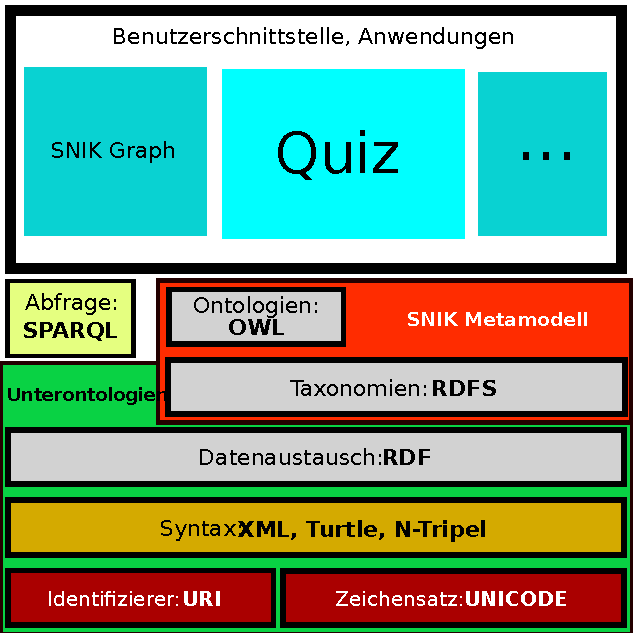
\includegraphics[width=0.7\textwidth]{images/swebstackde_snik.pdf}
\caption{Das semantische Modell von SNIK.}
\label{img:semanticwebstack2}
\end{figure}
Das Projekt konzentriert sich dabei hauptsächlich auf die Daten der medizinischen Lehre, um diese für Krankenhausinformationssysteme zur Verfügung zu stellen und die Arbeit für medizinisches Personal zu erleichtern, speziell hat der durch Prof. Dr. Alfred Winter geleitete Teilbereich \ac{MIG} die Zielsetzung, durch Entwicklung von Methoden und Werkzeugen für das Informationsmanagement zu einer besseren Gesundheitsversorgung beizutragen. Um normalen Nutzern eine Anwendung, die die Daten des Projektes nutzt, darzustellen, wurde unter anderem auch ein einfaches Multiple-Choice-Quiz auf Basis eines öffentlich verfügbaren Templates programmiert, was die Ontologie hinter SNIK nutzt, um Nutzern einfache, generierte Fragen zu stellen. 


\todo{
\begin{itemize}
\item In welcher Welt/Domäne oder welchem Arbeitsbereich/-gebiet bewegen wir uns im Rahmen der Seminararbeit/der ausgewählten Papers?
\item Worum geht es eigentlich?
\end{itemize}
Aus den Papers bzw. dem Antrag des Forschungsprojektes entnehmen.
}

\subsection{Problematik}
Da die Nutzer möglichst mit logischen, aber nicht zu einfachen Fragen herausgefordert werden sollten, um mithilfe des Multiple-Choice-Quiz ihren Wissensstand zu verbessern, sollte das Quizprogramm bestimmte Vorgaben erfüllen und diese auch in der Qualtität der Fragen widerspiegeln. 
\todo{
\begin{itemize}
\item Worin bestehen die Probleme?
\item Warum ist die geschilderte vorliegende Situation problematisch?
\item Für wen ist sie problematisch?
\end{itemize}
Aus den Papers bzw. dem Antrag des Forschungsprojektes entnehmen.\\
}
\todo{
Hier ist auf die generelle Problemlage einzugehen, die dem Aufsatz im Wissenschaftsfeld zu Grunde liegt.\\
Bsp.: Daten aus der Krankenversorgung stehen aus rechtlichen und technischen Gründen nicht für die Forschung zur Verfügung, sodass klinische Forscher eigene Datenerhebungen planen müssen.
}
\subsection{Motivation}
\todo{
\begin{itemize}
\item Warum lohnt es sich, die genannten Probleme zu lösen?
\item Wer wird welchen Nutzen von dieser Abschlussarbeit haben?
\item Warum sind die Papers wichtig?
\end{itemize}
Aus den Papers bzw. dem Antrag des Forschungsprojektes entnehmen.
}
\todo{
Worin liegt der zusätzliche Nutzen, die beiden Ansätze zu vergleichen? Worin liegt der Nutzen, den Ansatz des Papers auf die Problematik des Forschungsprojektes anzuwenden?\\
Bsp.: Gelänge es, Daten aus der Krankenversorgung vollständig zu anonymisieren, könnten sie für beliebige Forschungsvorhaben genutzt werden.
}

\section{Zielsetzung}
\todo{
Beschreiben Sie kurz die Zielsetzung ihrer Seminararbeit.
Beachten Sie dazu die Beschreibung des Betreuers zu Ihrem Seminarthema.\\
Beispiel:\\
Es soll herausgearbeitet werden, ob einer der in den Papers vorgestellten Lösungsansätze im aktuellen Forschungsprojekt angewendet werden kann: „Untersuchung der Eignung des Anonymisierungskonzept der statistischen Landesämter für medizinische Daten unter besonderer Betrachtung der Risiken des Zusatzwissens behandelnder Ärzte.“
Es soll eine Übersicht erarbeitet werden, die es ermöglicht, in einem konkreten Anwendungsfall den dort geeigneten Lösungsansatz auszuwählen.
}

\section{Vorgehensweise}
\todo{
Stellen Sie Ihre Methode bzw. Herangehensweise dar.
Was ist Ihre konkrete Aufgabenstellung im Rahmen der Seminararbeit? Das könnte z.B. sein:
\begin{itemize}
\item Vorstellen verschiedener Lösungsansätze, Vergleich und Bewertung der Lösungsansätze, Literaturrecherche nach weiteren vergleichbaren Papers.
\item Bewertung eines Lösungsansatzes hinsichtlich einer konkreten Forschungssituation.
Literaturrecherche nach weiteren vergleichbaren Papers.
\end{itemize}
}
\todo{
Beschreiben Sie Ihre Vorgehensweise in einzelnen Schritten und stellen Sie die Reihenfolge der Abarbeitung dar.
Auf diese Punkte sollten Sie in der Diskussion wieder eingehen.
}
\todo{
\begin{enumerate}
\item Schritt 1 
\item Schritt 2
\end{enumerate}
}
\todo{
Vermeiden Sie Formulierungen wie \enquote{Es ist nicht bekannt, ob...} oder \enquote{Es existiert kein...}.
Solche Formulierungen kehren in der Regel einfach das bereits angedachte Lösungsmodell um und postulieren das Fehlen der angedachten Lösung einfach als Problem.
... \\
Schritt n\\
Das ist ähnlich, wie wenn es in der Werbung hieße \enquote{Wenn Sie das Problem haben, dass Ihnen Aspirin fehlt, dann kaufen Sie doch Aspirin.}
Sinnvoller ist diese Aussage: \enquote{Wenn Sie das Problem haben, dass Ihnen der Kopf weh tut, dann kaufen Sie doch Aspirin.}
Es ist also bei der Problembeschreibung erforderlich, sich in die Lage dessen zu versetzen, den man mit der angedachten Lösung beglücken möchte.
Sein Problem ist zu ermitteln und so zu formulieren, er/sie das Problem wiedererkennt und dadurch geneigt ist, sich für die Lösung des Problems zu interessieren.
}

%\todo{(2--3 Seiten)}
\chapter{Grundlagen}
\todo{
Erklären Sie alle fachlichen Grundlagen, die notwendig sind, um der Bearbeitung Ihres Seminar­themas folgen zu können.
Beachten Sie, dass die Darstellung für den durchschnittlichen Vorlesungs­hörer verständlich ist.
}

\section{\acs{WWW}}
Das \ac{WWW} bildet ein verknüpftes Kommunikationsmodell zwischen allen Ressourcen und Nutzern des Internets, die das \ac{HTTP} nutzen.
Es wurde vom Direktor der \ac{W3C} Tim Berners-Lee 1991 entwickelt und ermöglicht den Zugriff auf sowie den Datenaustausch mit \acs{HTML}-Dokumenten.
Es definiert also das, was die Allgemeinheit als \enquote{das Web} bezeichnet.

\section{Semantic Web}
Das Semantic Web (oder auch: semantisches Netz) stellt eine Methode dar, um maschinenlesbares Wissen über das \ac{WWW} in Form von HTML-Dokumenten zu verbreiten.
Anders als bei der klassischen Website aber wird hier nicht nur primär Wert auf die Lesbarkeit durch einen Menschen, sondern auch auf die Maschinenlesbarkeit Wert gelegt, indem die Seite nebst dem normalen HTML-Code auch Informationen, die durch Computer gelesen werden können, hinterlegt. Diese sind durch Technologien des semantischen Webs ( \acs{RDF}, \acs{SPARQL}, ... ) einles- und verarbeitbar.

\section{Linked Data}
Der Begriff \enquote{Linked Data} bezieht sich auf eine Reihe bewährter Methoden zum Veröffentlichen und Verbinden strukturierter Daten im Web.
Es verknüpft Dateien aus dem semantischen Web untereinander, sodass sie durch semantische Abfragen benutzbar werden.
Linked Data basiert auf standardisierten Modellen für den Datenaustausch im Web, besipielsweise \acs{HTML}, um auch wie beim semantischen Prinzip maschinenlesbare Daten zu generieren.
Zielsetzung von Linked Data ist es, das Internet zu einer globalen, computerverbarbeitbaren Datenbank weiterzuentwickeln und so den Zugriff für technische Endgeräte weiter zu vereinfachen.

\section{\acs{RDF}}
\ac{RDF} ist ein weiteres Standardmodell für den Datenaustausch im Web, welches in den 90er Jahren des letzten Jahrtausends seine Anfänge findet.
Im Gegensatz zu \ac{HTML} und \ac{XML} ist es in der Lage, enthaltene Informationen zu kombinieren und weiter zu verarbeiten, anstatt diese nur korrekt anzuzeigen.
Daher ist RDF auch oft als grundlegendes Repräsentationsformat für die Entwicklung im Semantic Web angesehen.
Es erweitert die Verknüpfungsstruktur von diesem, um \ac{URIs} einzubinden.
Solche URIs werden im semantischen Netz dazu genutzt, Beziehungen zwischen Dingen beziehungsweise zwischen den beiden Enden der Verknüpfung herzustellen, um Dateien zu verknüpfen, verfügbar zu machen und für Anwendungen freizugeben.
Dadurch können Daten zusammengeführt werden, die sich eigentlich im Schema grundlegend unterscheiden, ohne dass alle Datenkonsumenten geändert werden müssen.
Diese Zusammenführung geschieht in einem Schichtenmodell: Aussagen werden als Tripel modelliert und bilden eine Aussage, die aus Subjekt, Prädikat und Objekt zusammengefügt werden kann.
Man kann also einen Tripel mit einem einfachen Satz vergleichen: als Beispiel hier einmal der Teilsatz \textit{Google produziert Prozessoren}.
Hier stellt \textit{Google} das Subjekt dar, \textit{produziert} ist das Prädikat und \textit{Prozessoren} sind das Objekt.
Hat man eine Menge von Tripeln, bilden diese ein semantisches Netz, was tabellarisch übersichtlich dargestellt werden kann, siehe \cref{tab:rdfexample}.

\begin{table}
\begin{centering}
\begin{tabularx}{\textwidth}{XXX}
\toprule
\textrm{Subjekt}			&\textrm{Prädikat}			&\textrm{Objekt}\\
\midrule
New York				&liegt in				&Amerika\\
Adobe				    &verkauft				&Software\\
Google					&produziert				&Prozessoren\\
\bottomrule
\end{tabularx}
\end{centering}
\caption{Beispiel für RDF-Tripel.}
\label{tab:rdfexample}
\end{table}


\section{\acs{SPARQL}}
\ac{SPARQL} ist ein Standard für die Abfrage von in \ac{RDF} spezialisierten Informationen sowie für die Darstellung der zugehörigen Resultate, siehe \cref{img:semanticwebstack1}.
Es basiert auf einfachen \ac{RDF}-Anfragen in Form von Graphmustern, also einer Menge von Tripeln, enthält jedoch auch erweiterte Funktionen für die Konstruktion komplexerer Anfragemuster, die Verwendung zusätzlich hinzufügbarer Filterbedingungen und für die Formatierung der schlussendlichen Ausgabe.


Man kann also \ac{SPARQL} als eine faktische Abfragesprache des semantischen Webs bezeichnen.
\begin{figure}
\centering
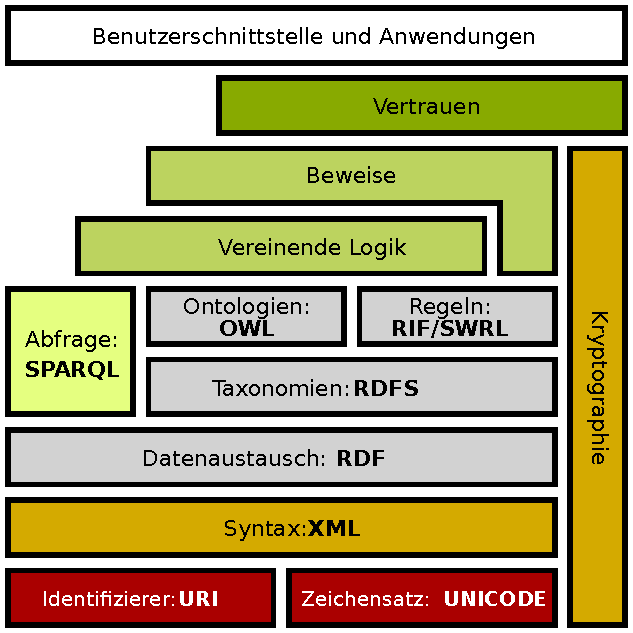
\includegraphics[width=0.7\textwidth]{images/swebstackde.pdf}
\caption{Der Semantic Web Stack.}
\label{img:semanticwebstack1}

\end{figure}
\section {Ontologien}
\setlength\epigraphwidth{.9\textwidth}
\setlength\epigraphrule{0pt}

\epigraph{\itshape An ontology is an explicit specification of a conceptualization.}{---Thomas R. Gruber\todo{quelle zitieren}}

\noindent Ontologien sind (im informatischen Kontext) meist sprachlich gefasste und geordnete Darstellungen einer Menge von Begrifflichkeiten mit festen Beziehungen untereinander.
Diese Beziehungen befassen sich stets auf einen bestimmten Gegenstandsbereich und werden dazu genutzt, Wissen in digitalisierter Form zwischen Anwendungen und Diensten auszutauschen.
Dabei müssen bestimmte Interferenz- und Integritätsregeln eingehalten werden, also Regeln zu Schlussfolgerungen sowie zu der Gewährleistung ihrer Gültigkeit.
Ontologien erfreuen sich seit der Idee des semantischen Webs einem stets wachsenden Bekanntheitsgrad, was dazu führt, dass sie als Teil der Wissensrepräsentation im Teilgebiet \acs{KI} einen großen Einfluss haben.
Dabei beschreibt die Idee des Semantic Web eine Erweiterung des vorhandenen Netzes, um Daten zwischen Rechnern einfacher austausch- und verwertbar zu machen und sie somit besser zu explizieren, anstatt sie unkonstruiert stehen zu lassen.
Zum Sinne dieser Realisierung dienen Standards zur Veröffentlichung und Nutzung maschinenlesbarer Daten -- insbesondere \ac{RDF}.

\section{Künstliche Intelligenz}
\ac{KI} ist ein Teilgebiet der Informatik, welches sich mit der Automatisierung intelligenten Verhaltens befasst.
Es spiegelt eine Möglichkeit wieder, bestimmte Entscheidungsstrukturen des Menschen nachzubilden und es somit Computern zu ermöglichen, komplexe Probleme selbstständig zu bearbeiten und zu lösen.
Um diese Informationen weiter zu nutzen, können Methoden des Semantic Web genutzt werden, um sie als Tripel einfach maschinenlesbar darzustellen und für andere Computer verfügbar zu machen.
\section{\acs{SNIK}-Projekt}
Das \ac{SNIK} ist ein vollendetes Projekt, welches Begriffe des Informationsmanagements sowie deren Beziehungen untereinander beschreibt.
Es ist in der Lage, diese Menge an Informationen in einer Ontologie darzustellen und diese sowie maschinen- als auch menschenlesbar auszugeben.
 Dabei nutzt es ein dem Semantic Web Stack ähniches Modell(\cref{img:semanticwebstack2}), welches Anwendungen wie dem \ac{SNIK} Graph oder einem Multiple-Choice-Quiz ermöglicht, Informationen abzufragen und diese Endnutzern in aufbereiteter Form zur Verfügung zu stellen.
Dabei konzentriert sich das SNIK-Projekt hauptsächlich auf die Daten der medizinischen Lehre, um diese für Krankenhausinformationssysteme zur Verfügung zu stellen und die Arbeit für medizinisches Personal zu erleichtern.
\begin{figure}
\centering
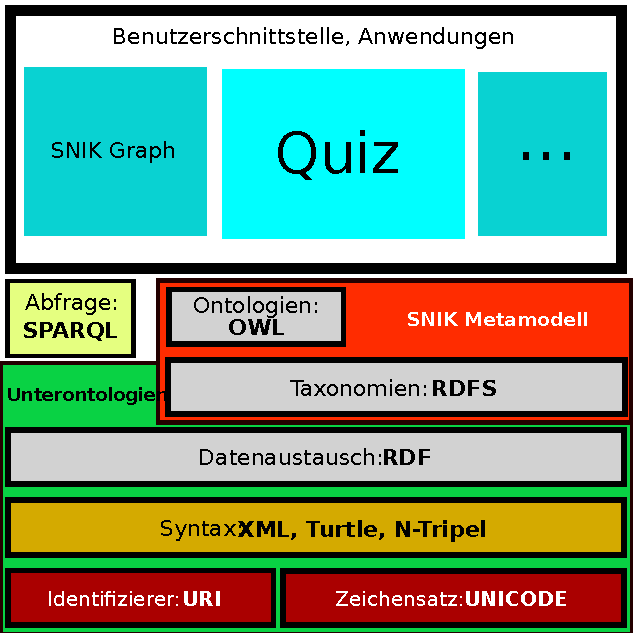
\includegraphics[width=0.7\textwidth]{images/swebstackde_snik.pdf}
\caption{Das semantische Modell von SNIK.}
\label{img:semanticwebstack2}
\end{figure}

\section{Krankenhausinformationssysteme}
\paragraph{Informationssystem}
Ein Informationssystem ist ein System, welches durch die Bildung logischer Zusammenhänge eine Deckung der Informationsnachfrage zur Aufgabe hat.
Es produziert, beschafft, verteilt und verarbeitet Daten durch eine Zusammenarbeit zwischen Mensch und Technik durch Aufgaben.
\paragraph{Krankenhausinformationssystem}
Krankenhausinformationssysteme beschreiben die Gesamtheit aller Informationssysteme zur Produktion, Beschaffung, Verteilung und Verarbeitung von medizinischen und administrativen Daten im Krankenhaus.
Dazu gehören verschiedene Formen der Datenbereitstellung sowie auch konventionelle Methoden der papierbasierten Dokumentation und der sprachlichen Kommunikation.
Das grundsätzliche Ziel eines Krankenhausinformationssystems ist, die Kommunikation zwischen Mitarbeitern zu verbessern und den Ablauf in Krankenhäusern zu steuern, indem Mitarbeitern gezielt Zugriff auf für ihn relevantes Wissen aus der ihm zugeteilten Benutzerrolle gegeben wird, zum Beispiel über den gerade zu behandelnden Patienten.
\paragraph{Wissen}
Wissen ist die Kenntnis über den in einem Fachgebiet zu gegebener Zeit gegebenen Konsens, vor allem bezogen auf eine gültige Terminologie, erlaubte Interpretationen, bestehender Zusammenhänge und Gesetzmäßigkeiten sowie empfehlenswerter Methoden und Handlungen.
Wissen ist also auch Information, aber in dem Fall nicht auf einzelne Objekte, sondern eine Menge von Objekten und deren Beziehungen untereinander bezogen, vgl. \citet{his}.
\paragraph{Daten}
Daten sind Gebilde aus Zeichen oder kontinuierliche Funktionen, die durch bekannte oder unterstellte Beziehungen Informationen darstellen können.
Sie stellen die Grundlage oder das Ergebnis eines Verarbeitungsschrittes dar. 
\chapter{Lösungsansatz/Lösungsansätze \todo{(2--4 Seiten)}}
\todo{Kapitel 3 ist Vorschlag gedacht, der nicht wörtlich übernommen werden muss.
Der Lösungsansatz ist eine kurze Beschreibung der Arbeitshypothese sowie des Vorgehens zur Lösung der in der Einleitung beschriebenen Probleme.}

%Beispiel-Query:
\begin{comment}
\begin{lstlisting}
SELECT SAMPLE(replace(str(?def),str(?cl),"X","i") as ?def)
SAMPLE(str(?cl) as ?cl) 
SAMPLE(str(?a1l) as ?a1l)
SAMPLE(str(?a2l) as ?a2l)
SAMPLE(str(?a3l) as ?a3l)
{
 ?class a owl:Class.
 ?class rdfs:label ?cl.
 FILTER(LANGMATCHES(LANG(?cl),"en"))

 ?class skos:definition ?def.
 FILTER(STRLEN(?def)>10&&STRLEN(?def)<600).
 FILTER(LANGMATCHES(LANG(?def),"en"))

 ?class (!meta:subTopClass){1,2} ?a1,?a2,?a3.

 owl:Class ^a ?a1,?a2,?a3.
 FILTER(?class!=?a1&&?class!=?a2&&?class!=?a3
 &&?a1<?a2&&?a2<?a3)

?a1 rdfs:label ?a1l.
 FILTER(LANGMATCHES(LANG(?a1l),"en"))

?a2 rdfs:label ?a2l.
 FILTER(LANGMATCHES(LANG(?a2l),"en"))

?a3 rdfs:label ?a3l.
 FILTER(LANGMATCHES(LANG(?a3l),"en"))
 
} GROUP BY ?class limit 1000
\end{lstlisting}
\end{comment}

\section{Ergebnis/Lösungsansatz Paper n}
\section{Vergleich mit Projekt}

\chapter{Ergebnis \todo{der Seminararbeit, 1--2 Seiten, ihre Ergebnisse}}
\todo{
Im Ergebniskapitel soll beschrieben werden, inwiefern Sie Ihre in 1.2/1.3 aufgestellten Ziele bzw. Aufgaben im Rahmen der Seminararbeit erreicht wurden oder auch weshalb sie (teilweise) nicht erreicht werden konnten.
So soll es möglich sein, dass ein Leser von der Arbeit lediglich die Einleitung und die Zusammenfassung liest und doch die Ergebnisse der Arbeit erfassen kann.
Dieses Kapitel kann auch in mehrere Unterkapitel aufgeteilt werden, wenn das sinnvoll ist!
}

\chapter{Diskussion und Ausblick \todo{1--2 Seiten}}
\todo{
In der Diskussion wird das Ergebnis der Arbeit noch einmal kritisch bewertet.
Dies umfasst auch neue Probleme, die erst während der Bearbeitung erkannt wurden.
Die Eignung für ein konkretes Forschungsprojekt sollte hier diskutiert werden.
In der Diskussion kann auch die Kritik des Autors an dem stehen, was er in der Literatur zu dem zu bearbeitenden Thema hier und da gelesen hat.
Außerdem soll ein Ausblick gegeben werden, welche weiteren Fragestellungen noch bearbeitet werden sollten.
}

\renewcommand{\bibpreamble}{
\todo{
Zentrale Literatur, die den untersuchten Artikeln zugrunde liegt, können Sie im bibtex-Format in die seminar.bib einfügen und dann im Text zitieren, wodurch diese automatisch in das Literaturverzeichnis übernommen werden.
Sie können auch weitere referierte Veröffentlichungen (wissenschaftliche Zeitschriften (auch elektronisch), Bücher) in die Erarbeitung einbeziehen zitieren.
Sie können dafür Literaturdatenbanken wie Pubmed oder Google Scholar durchsuchen und dort direkt als bibtex-Eintrag herunterladen.
Bitte beachten Sie, dass die \href{https://www.openoffice.org/bibliographic/bibtex-defs.html}{bibtex-Einträge vollständig sind}, z.B. sind das bei Büchern Autor, Editor, Title, Kapitel oder Seiten, Herausgeber und Jahr..
Weitere Informationen zum Thema der Literaturrecherche finden sich in den \href{http://www.imise.uni-leipzig.de/Lehre/MedInf/Abschlussarbeiten/Literaturrecherche.jsp}{Hinweisen zur Literaturrecherche}.
\paragraph{Beispielzitierungen}
\citet{his} beschreiben ein Verfahren zur X von Y auf Basis von Z.
Alternativ: X von Y lässt sich auf Basis von Z ermitteln~\citep{his}.
}
}

\bibliographystyle{dinat}
\bibliography{bell}

\end{document}

